%\documentclass[a4paper, draft]{article}
\documentclass[a4paper]{article}

% A new package for bibliography
% Use biber for bibtex and pdflatex instead of latex
\usepackage[backend=biber]{biblatex}
% new from biblatex
\addbibresource{/home/jorgsk/phdproject/bibtex/jorgsk.bib}

% Support for unicode
\usepackage[utf8]{inputenc}
\usepackage[T1]{fontenc}

\usepackage{amsmath,amsfonts,amssymb,amsthm,booktabs,array,mathtools,mhchem}
% consider package mhchem for typesetting chemical formulas

% Proper space and font for integral differential term
\newcommand{\te}[1]{\text{#1}} 
\newcommand{\dd}{\; \mathrm{d}} 
% Shorcut for ODEs with proper font
\newcommand{\diff}[2]{\frac{\mathrm{d} #1}{\mathrm{d} #2}}
% Shortcut for PDEs with proper font (shortcut: PDB)
\newcommand{\pdiff}[2]{\frac{\partial #1}{\partial #2}}
\newcommand{\pdiffn}[3]{\frac{\partial^{#3} #1}{\partial #2^{#3}}}

% Absolute value and norm commands.
% Read the mathtools.pdf to fix these!
\providecommand{\abs}[1]{\lvert#1\rvert} 
\providecommand{\norm}[1]{\lVert#1\rVert}

% Set the depth of section numbering
\setcounter{secnumdepth}{0}

\begin{document} 
\noindent

\subsection{Chemical equation for RNAP movement}

Below is a reaction equation for the RNA polymerase as it is translocating on
DNA.
\begin{align}
\ce{R_i^{\text{e}}
<=>
R_i^{\text{s}}
<=>
R_i^{\text{s}}N_t
<=>
R_{i+1}^{\text{e}}
+ PP_i
}
\label{eq:full}
\end{align}
\\
The following terms are used in equation \eqref{eq:full}:
\begin{itemize}
	\item $\te{R}_i^{\te{e}}$ is the pre-translocated polymerase at nucleotide $i$
	\item $\te{R}_i^{\te{s}}$ is the post-translocated polymerase at nucleotide $i$
	\item $\te{R}_{i+1}^{\te{e}}$ is the pre-translocated polymerase at nucleotide $i+1$
	\item $\te{N}_{\te{t}}$ is the incoming NTP
	\item $\te{PP}_i$ is the released $\te{PP}_i$ from nucleotide incorporation
\end{itemize}
See also Figure 1 adopted from the Landick paper (Hein \textit{et al.}) for what these symbols
represent.
\begin{figure}[h]
  \centering
    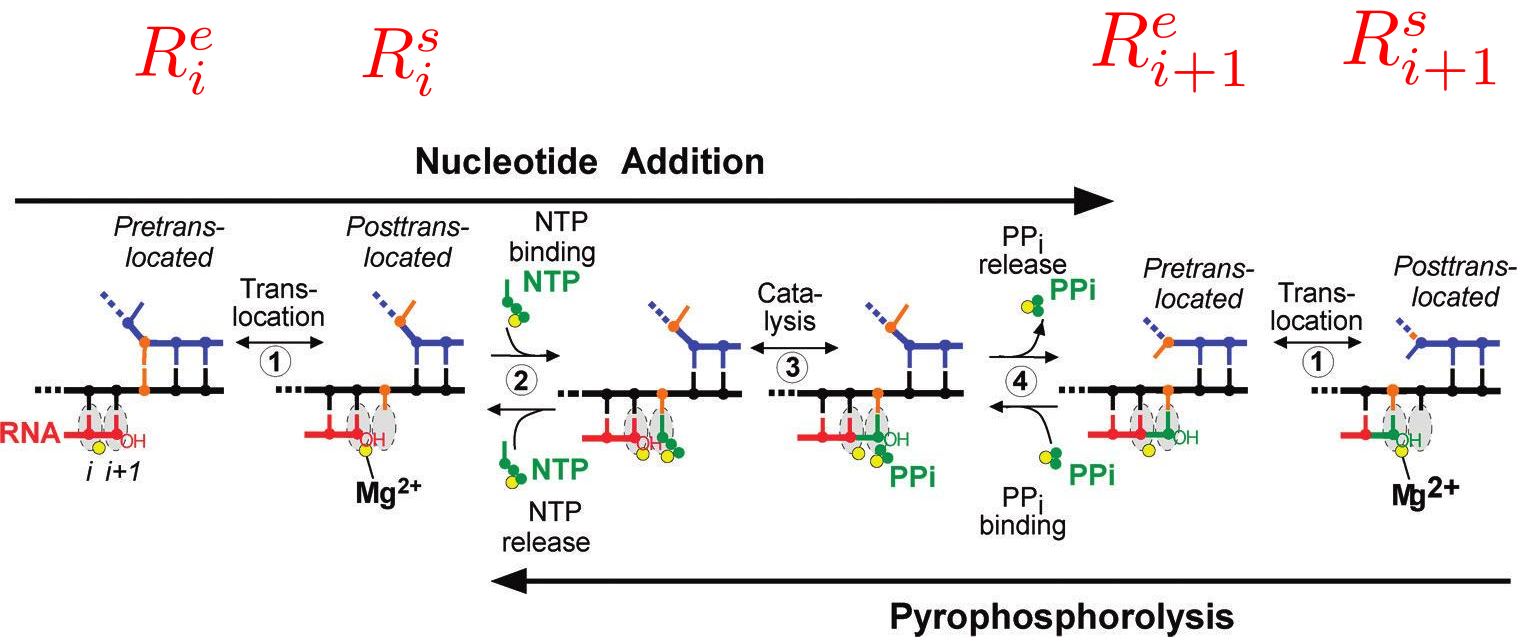
\includegraphics[scale=0.3]{images/modifiedLandick}
	\caption{Polymerase at pre-translocated and post-translocated states for
	nucleotides $i$ and $i+1$}
\end{figure}

$i$ refers to the length of the growing RNA. Since backtracking is not
included, this is equivalent to the template position at the active site. All
expressions (like $\te{R}_i^{\te{e}}$) should be interpreted as concentrations
($mmol/L$ for example).

In the reaction equation \eqref{eq:full} RNAP moves between the pre-translocated and the
post-translocated step at some nucleotide position $i$. In the
post-translocated step, a nucleotide $\te{N}_{\te{t}}$ may bind in the active
site. This nucleotide may then be incorporated, bringing RNAP to position
$i+1$ and at the same time releasing $\te{PP}_i$. This reaction ignores all
pathways related to backtracking and abortion.

To make a model fit for simulation, we want to simplify the reaction kinetics.
The first simplifying assumption is to make the nucleotide binding and
synthesis step implicit:
\\
\begin{align}
\ce{R_i^{\text{e}}
<=>
R_i^{\text{s}}
<=>
R_{i+1}^{\text{e}}.
}
\label{eq:reduced3}
\end{align}
\\
Next, we assume that PPi binding is negligible. Then we reach the
following simplified reaction
\\
\begin{align}
\ce{R_i^{\text{e}}
<=>
R_i^{\text{s}}
->[\ce{k1_i}]
R_{i+1}^{\text{e}}.
}
\label{eq:reduced33}
\end{align}
\\
Here, the reaction rate $k_1$ is the rate of the nucleotide incorporation step.

To simplify further, we assume that the step between pre-translocation and
post-translocation reaches equilibrium. This assumption is not likely to be
true, but we perform it in order to be able to introduce the $Keq$ parameter
into our equation and to simplify the model. Even though the assumption is not
be entirely true, we only need that it is approximately true. We sacrifice some
accuracy in order to have a more simplified model. The reaction we end up with
is then:
\\
\begin{align}
\ce{R_i^{\text{e}}
<=>[\ce{Keq_i}]
R_i^{\text{s}}
->[\ce{k1_i}]
R_{i+1}^{\text{e}}.
}
\label{eq:reduced4}
\end{align}
\\
Here $Keq_i$ is the assumed equilibrium constant for the translocation step:
\begin{equation}
	\te{R}_i^{\te{s}} = \frac{\te{R}_i^{\te{e}}}{Keq_i}
	\label{eq:keq}
\end{equation}
We will use only the last reaction step in our model:
\\
\begin{align}
\ce{R_i^{\text{s}}
->[\ce{k1_i}]
R_{i+1}^{\text{e}}
}
\label{eq:reduced5}
\end{align}
\subsection{From chemical equation to differential equation}
The rate equation for equation \eqref{eq:reduced5} is by definition:
\begin{equation*}
	r = k_{1_i}R_i^{\text{s}}
\end{equation*}
Since the rate is the change of $R_{i+1}^{\text{e}}$ with time,
we form the differential equation
\begin{equation*}
	\diff{R_{i+1}^{\text{e}}}{t} = k_{1_i}R_i^{\text{s}}
\end{equation*}

Now we can make use of the relationship in equation \eqref{eq:keq} and write
\begin{equation}
	\diff{R_{i+1}^{\text{e}}}{t} = k_{1_i}\frac{[\te{R}_i^{\te{e}}]}{Keq_i}
	\label{eq:nice}
\end{equation}
\\
So far, by making a series of simplifying steps, we have arrived at an equation
that relates the concentration of RNAP at position $i+1$ to the concentration
of RNAP at position $i$. The next question is, what does $k_1$ look like? A
general expression for the rate of a reaction is the following:
\begin{equation*}
	k_1 = Ke^{-\frac{\Delta G}{RT}},
\end{equation*}
where $\Delta G$ is the Gibbs free energy change associated with the reaction,
$R$ is the universal gas constant and $T$ is the temperature in Kelvin. By
inserting this expression into equation \eqref{eq:nice}, we get
\begin{equation*}
	\diff{\te{R}_{i+1}^{\te{e}}}{t} = Ke^{-\frac{\Delta G}{RT}}\frac{\te{R}_i^{\te{e}}}{Keq_i}
\end{equation*}
Now we have exponential we initially sought. We need to get $Keq$ into that exponential. By using
\begin{equation*}
	Keq_i = e^{\te{ln}(Keq_i)} \ (\te{from} \ x = e^{ln(x)})
\end{equation*}
we obtain
\begin{align*}
	\diff{\te{R}_{i+1}^{\te{e}}}{t} &= \frac{Ke^{-\frac{\Delta
	G}{RT}}\te{R}_i^{\te{e}}}{e^{ln(Keq_i)}}\\
	&= Ke^{-\frac{\Delta G}{RT} - ln(Keq_i)}\te{R}_i^{\te{e}}
\end{align*}

The term $RT$ evaluates to 0.62. Thus we have 
\begin{equation}
	\diff{\te{R}_{i+1}^{\te{e}}}{t} \sim e^{-1.6\Delta G - \te{ln}(Keq)}
	\label{eq:stuff}
\end{equation}
which is a term very similar to what we started out with, which was:
\begin{equation*}
	e^{\Delta G_{\text{RNA-DNA}} - Keq}
\end{equation*}

\subsection{Intermission}
By performing some simplifying assumptions on the reaction \eqref{eq:full}, we
have arrived at a term for the rate of RNAP elongation that is similar to the
term we originally started with.

The biggest difference between the two expressions is in the sign of $\Delta
G_{\text{RNA-DNA}}$. The difference between $log(Keq)$ and $Keq$ is not large
since the values for $Keq$ are around 1 ($log(x)$ is approximately linear around $x = 1$).

To test if this simplified model would work at all, I simulated a set of
ordinary differential equations based on equation \eqref{eq:stuff}, using
$\Delta G_{\text{RNA-DNA}}$ in place of $\Delta G$. I get a nice correlation
$(r = 0.7)$ -- except that I must change the sign of $\Delta
G_{\text{RNA-DNA}}$ from negative to positive.  Otherwise the correlation
breaks down.

The fact that the $\Delta G$ term from equation \eqref{eq:stuff} has a positive
instead of a negative sign, indicates that this term is working to 'hold back'
the reaction. A candidate for the $\Delta G$ term other than $\Delta
G_{\text{RNA-DNA}}$ is the one involved with scrunching of DNA during
initiation. The $\Delta G_{\text{DNA-DNA}}$ energies are similar to the $\Delta
G_{\text{RNA-DNA}}$ energies but not identical. The next challenge is to try to
incorporate DNA scrunching into the model.

\subsection{Scrunching}
To introduce scrunching into the model, the following assumptions are made
about the physics of transcription initiation
\begin{enumerate}
	\item the RNA-DNA hybrid acts to stabilize the initiation complex
	\item the scrunched DNA-DNA bubble de-stabilizes the initiation complex
	\item the $\Delta G_{\text{RNA-DNA}}$ and $\Delta G_{\text{DNA-DNA}}$
		energies were obtained for helical conformations; how these parameters
		are applicable to the RNA-DNA hybrid and the scrunched DNA bubble is not straightforward
	\item modeling the non-abortive pathway of transcription initiation is a
		good enough approximation to describe the system
\end{enumerate}
Let us now revisit equation \eqref{eq:stuff}:
\begin{equation*}
	\diff{\te{R}_{i+1}^{\te{e}}}{t} \sim e^{-\frac{\Delta G}{RT} - \te{ln}(Keq)}
\end{equation*}
The $\Delta G$ term is the free energy term that (together with the value of
$Keq$) determines if the reaction
\begin{align*}
\ce{R_i^{\text{s}}
->[\ce{k1_i}]
R_{i+1}^{\text{e}}
}
\end{align*}
will take place. Based on assumptions 1 and 2 in the above list, we propose
that this energy term is on the following form:
\begin{equation*}
	%\Delta G = \Delta G_{\te{Stabilizing}} - \Delta G_{\te{Destabilizing}} +
	%\Delta G_{\te{Initiation}}
	\Delta G = \Delta G_{\te{Stabilizing}} - \Delta G_{\te{Destabilizing}}
\end{equation*}
where
\begin{itemize}
	\item $\Delta G_{\te{Stabilizing}}$ is the $\Delta G_{\te{RNA-DNA}}$ energy
		of the growing RNA-DNA hybrid
	\item $\Delta G_{\te{Destabilizing}}$ is the $\Delta G_{\te{DNA-DNA}}$ energy
		of the scrunched DNA bubble
	%\item $\Delta G_{\te{Initiation}}$ is the $\Delta G_{\te{RNA-DNA}}$ energy
		%for incorporation of the incoming nucleotide
\end{itemize}
However, as stated in assumption 3, we do not know the relationship between the
measured values of $\Delta G_{\te{RNA-DNA}}$ and $\Delta G_{\te{DNA-DNA}}$ from
the literature, and the role these values play in transcription initiation. As
a first approximation, we assume that the values in transcription initiation
correspond to a simple scaling of the measured values by multiplying factor.
Thus, we rewrite equation \eqref{eq:stuff} to obtain:
\begin{equation}
	%\diff{\te{R}_{i+1}^{\te{e}}}{t} \sim e^{\frac{-c1\Delta
	%G_{\te{Stabilizing}} - c2\Delta G_{\te{Destabilizing}} +
	%c3\Delta G_{\te{Initiation}} }{RT} - \te{ln}(Keq)}
	\diff{\te{R}_{i+1}^{\te{e}}}{t} \sim e^{\frac{-c1\Delta
	G_{\te{Stabilizing}} - c2\Delta G_{\te{Destabilizing}}}{RT} - \te{ln}(Keq)}
	\label{eq:bigmodel}
\end{equation}
%In this model, the term $c1\Delta G_{\te{Stabilizing}} - c2\Delta
%G_{\te{Destabilizing}} + c3\Delta G_{\te{Initiation}}$ will be positive during
In this model, the term $c1\Delta G_{\te{Stabilizing}} - c2\Delta
G_{\te{Destabilizing}}$ will be positive during
transcription initiation, at least for $c1$ and $c2$ equal to 1. We have thus
found a way of including 'scrunching' in the model in such a way that the sign
of the $\Delta G$ term is positive.

\subsection{Interpretation of $\Delta G$ in transcription initiation}
The starting value for the $\Delta G_{\te{Stabilizing}}$ term will be 0 (hybrid of
length 0), and the starting value for $\Delta G_{\te{Destabilizing}}$
will be equal to that of the ~13 bp initial bubble. As initiation proceeds, the
$\Delta G_{\te{Stabilizing}}$ will grow (hybrid increases in size), but the
term will be more or less equalized by the growth of the $\Delta
G_{\te{Destabilizing}}$ term (the growth of the bubble). Only after the RNA-DNA
hybrid has reached 8-9 basepairs will the $\Delta G_{\te{Stabilizing}}$ term
stop to grow. From here on, $\Delta G$ will be come increasingly positive as
the DNA-DNA bubble continues the grow but the RNA-DNA hybrid remains
constant.

It is possible that the $\sigma$ barriers at 9 and 15 nt should be
implemented in the model, but it's not clear how this should be done.

\subsection{Conclusion}
I will now try to model equation \eqref{eq:bigmodel} and see if this model fits
the data.

% new from biblatex
%\printbibliography

\end{document}


